\documentclass[12pt]{exam}

% essential packages
\usepackage{fullpage} % margin formatting
\usepackage{enumitem} % configure enumerate and itemize
\usepackage{amsmath, amsfonts, amssymb, mathtools} % math symbols
\usepackage{xcolor, colortbl} % colors, including in tables
\usepackage{makecell} % thicker \Xhline in table
\usepackage{graphicx} % images, resizing

% sometimes needed packages
\usepackage{hyperref} % hyperlinks
\usepackage{tikz} % drawing graphs
\usetikzlibrary{positioning}

% paragraph formatting
\setlength{\parskip}{6pt}
\setlength{\parindent}{0cm}

% newline after Solution:
\renewcommand{\solutiontitle}{\noindent\textbf{Solution:}\par\noindent}

% less space before itemize/enumerate
\setlist{topsep=0pt}

% creates \filcl to grey out cells for groupwork grading
\newcommand{\filcl}{\cellcolor{gray!25}}

% creates \probnum to get the problem number
\newcounter{probnumcount}
\setcounter{probnumcount}{1}
\newcommand{\probnum}{\arabic{probnumcount}. \addtocounter{probnumcount}{1}}

% use roman numerals by default
\setlist[enumerate]{label={(\roman*)}}

% creates custom list environments for grading guidelines, question parts
\newlist{guidelines}{itemize}{1}
\setlist[guidelines]{label={}, left=0pt .. \parindent, nosep}
\newlist{gwguidelines}{enumerate}{1}
\setlist[gwguidelines]{label={(\roman*)}, nosep}
\newlist{qparts}{enumerate}{2}
\setlist[qparts]{label={(\alph*)}}
\newlist{qsubparts}{enumerate}{2}
\setlist[qsubparts]{label={(\roman*)}}
\newlist{stmts}{enumerate}{1}
\setlist[stmts]{label={(\roman*)}, nosep}
\newlist{pflist}{itemize}{4}
\setlist[pflist]{label={$\bullet$}, nosep}
\newlist{enumpflist}{enumerate}{4}
\setlist[enumpflist]{label={(\arabic*)}, nosep}

\printanswers

\newcommand{\prevhwnum}{7}
\newcommand{\hwnum}{8}

\begin{document}
%%%%%%%%%%%%%%% TITLE PAGE %%%%%%%%%%%%%%%
\title{EECS 203: Discrete Mathematics\\
  Winter 2024\\
  Homework \hwnum{}}
\date{}
\author{}
\maketitle
\vspace{-50pt}
\begin{center}
  \huge Due \textbf{Thursday, April 4}, 10:00 pm\\
\Large No late homework accepted past midnight.\\
\vspace{10pt}
\large Number of Problems: $8+2$
\hspace{3cm}
Total Points: $100+30$
\end{center}
\vspace{25pt}
\begin{itemize}
    \item \textbf{Match your pages!} Your submission time is when you upload the file, so the time you take to match pages doesn't count against you.
    \item Submit this assignment (and any regrade requests later) on Gradescope. 
    \item Justify your answers and show your work (unless a question says otherwise).
    \item By submitting this homework, you agree that you are in compliance with the Engineering Honor Code and the Course Policies for 203, and that you are submitting your own work.
    \item Check the syllabus for full details.
\end{itemize}
\newpage
%%%%%%%%%%%%%%% TITLE PAGE %%%%%%%%%%%%%%% 

\section*{Individual Portion}

\subsection*{\probnum Easy Peasy Degree-sy Squeezy [8 points]}
Let $G$ be a graph with $v$ vertices and $e$ edges. Let $M$ be the maximum degree of the vertices of $G$, and let $m$ be the minimum degree of the vertices of $G$. Show that
\begin{qparts}
    \item $\dfrac{2e}{v} \geq m$
    \item $\dfrac{2e}{v} \leq M$
\end{qparts}

\begin{solution}
    \begin{qparts}
        \item The total degree of the vertices is $2e$, since each edge is counted twice by its two vertices. 
        \par Let every vertex have $2e$ "vacancies," that is, spots for edges to fill. (Essentially, for each vertex, this "vacancy" number is just the difference between $2e$ and the degree of that vertex.) Then there will be $2ev$ "vacancies" total among the vertices, before edges fill them. After subtracting the edges, there will be $2ev - 2e$ total "vacancies" left among the edges. Let the pigeons be the "vacancies" and the vertices be the holes. Then by the Pigeonhole Principle, there must be at least one vertex with at least $\frac{2ev - 2e}{v} = 2e - \frac{2e}{v}$ ``vacancies.'' This translates to a degree of $2e - \left(2e - \frac{2e}{v}\right) = \frac{2e}{v}$. So there is at least one vertex with degree at most $\frac{2e}{v}$. Since the minimum degree must be less than or equal to this, $\dfrac{2e}{v} \geq m$.
        \item The total degree of the vertices is $2e$, since each edge is counted twice by its two vertices. There are $v$ vertices (holes) and $2e$ total degree (pigeons). So by the pigeonhole principle, there is one vertex with degree at least $\dfrac{2e}{v}$. Since the maximum degree must be greater than or equal to this degree, $\dfrac{2e}{v} \leq M$.
    \end{qparts}
\end{solution}

\clearpage

\subsection*{\probnum The Forest Beyond the Trees [15 points]}
Determine which of the following graphs is/are a tree. Additionally, determine which of the following graphs is/are bipartite. Please explain your reasoning for why each one is or is not a tree, and why each one is or is not bipartite.
\begin{qparts}
    \item $C_4,$ a cycle of length 4
    \item ~\\
    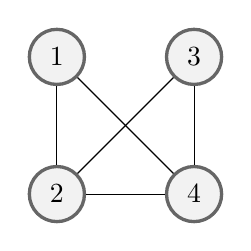
\begin{tikzpicture}[
    roundnode/.style={circle, draw=black!60, fill=gray!10, very thick, minimum size=7mm},
    ]
    %Nodes
    \node[roundnode] (1) {1};
    \node[roundnode] (2) [below=of 1] {2};
    \node[roundnode] (3) [right=of 1] {3};
    \node[roundnode] (4) [below=of 3] {4};
    
    \draw[-] (3)--(4);
    \draw[-] (2)--(3);
    \draw[-] (4)--(2);
    \draw[-] (2)--(1);
    \draw[-] (1)--(4);
    \end{tikzpicture}

    \item $K_6$
    \item ~\\\includegraphics[scale = 0.8]{images/08-2d.png}
    \item ~\\\includegraphics[scale = 0.8]{images/08-2e.png}
\end{qparts}

\begin{solution}
    \begin{qparts}
        \item This is not a tree since it contains a cycle subgraph. However, it is bipartite since it doesn't have a odd cycle.
        \item This is not a tree since it contains cycle subgraphs (e.g. the cycle of nodes 1-2-4). Additionally, it is not bipartite since it contains odd cycles. (e.g. the cycle of nodes 1-2-4).
        \item This is not a tree since it contains many cycle subgraphs. It is also not bipartite since it contains odd cycles. (Since it is complete, there is a cycle between any set of vertices, e.g. vertices 1, 2, 3)
        \item This is a tree because it contains no cycles. Additionally, since it does not contain any cycles, it does not contain odd cycles, and so it is bipartite.
        \item This is not a tree because it contains a cycle from a-b-d-g. However, since it does not contain any odd cycles, it is bipartite.
    \end{qparts}
\end{solution}

\newpage
\subsection*{\probnum Road Rage [12 points]}
The graphs below shows some major roads in New Jersey. The graph on the left shows distances between cities on these roads, and the graph on the right shows the toll costs on each road.

\resizebox{\textwidth}{!}{
\includegraphics[]{images/08-3.png}
}

For each pair of cities below, (i) find the shortest path in distance, and (ii) find the least expensive route (shortest path in terms of cost). Be sure to list the total distance and total cost for each respective part.

\begin{qparts}
    \item Newark to Camden
    \item Trenton to Atlantic City
\end{qparts}

\begin{solution}
    \begin{qparts}
        \item \begin{qsubparts}
            \item Must take Newark to Woodbridge: +20 \\
            \par Next, we compare routes from Woodbridge to Camden. Camden is connected to Trenton, Woodbridge, and Atlantic City. Cape May is not an option since its path from Woodbridge is very clearly longer than the others. \\
            Direct Woodbridge-Camden: +60 \\
            Woodb.-Trenton-Camden: $>60$ \\
            Woodb.-Asbury-Trenton(-Camden): $>60$ \\
            Woodb.-Asbury-Atlantic(-Camden): $>60$ \\
            \par So Newark-Woodbridge-Camden is the shortest path by distance, with a length of $60+20 = 80$.
            \item Again, must take Newark to Woodbridge: +\$0.60. Also, direct Woodbridge to Cambridge is free, so it is the cheapest from Woodbridge to Cambridge. So the cheapest path is Newark-Woodbridge-Camden, for a total of \$0.60.
        \end{qsubparts}
        \item \begin{qsubparts}
            \item Trenton - Camden - Atlantic City: $30 + 55 = 85$
            \item Trenton - Ashbury Park - Atlantic City: $0.00 + 1.25 = \$ 1.25$.
        \end{qsubparts}
    \end{qparts}
\end{solution}

\newpage
\subsection*{\probnum Isomorphish? [12 points]}
Determine whether or not each of the following pairs of graphs are isomorphic. If yes, provide an isomorphism. If not, explain why and propose a change to one of the graphs that would make them isomorphic; you do not need to provide an isomorphism in this case.
\begin{qparts}
    \item ~\\\includegraphics[width=14cm]{images/08-4a.png}
    \item ~\\\includegraphics[width=14cm]{images/08-4b.png}
\end{qparts}

\begin{solution}
    \begin{qparts}
        \item Yes. The isomorphism $f$ which maps
        \begin{align*}
            f(1) &= b \\
            f(2) &= e \\
            f(3) &= d \\
            f(4) &= c \\
            f(5) &= a
        \end{align*}
        \item No. On the left side, there is a single node with a degree of 5, vertex 7. However, on the right side, there are two such vertices: a and d.
        \par However, the left side could be made isomorphic to the right side by adding an edge from vertex 6 to vertex 3.
    \end{qparts}
\end{solution}

\newpage

\subsection*{\probnum Any tours available? [12 points]}
State whether each of the following contains, or is guaranteed to contain a Hamiltonian Cycle. Justify your response for each part. 
\begin{qparts}
    \item ~\\\includegraphics[width=3cm]{images/08-5a.png} 
    \item ~\\\includegraphics[width=7.5cm]{images/08-5b.png} 
    \item A simple, bipartite graph with 4 vertices that contains one cycle
    \item A 4-vertex graph where each vertex has even degree 
\end{qparts}

\begin{solution}
    \begin{qparts}
        \item Yes. The path from a-b-d-c-e-a.
        \item No. There is no way to return to a node on either side because the c-f edge can only be traveled once.
        \item Yes. The graph must contain an even cycle since it is bipartite. Also, because it is simple, there cannot be a 2-cycle. So the cycle must be a 4-cycle, which would contain all the vertices, and be a path for a Hamiltonian cycle.
        \item No. The graph can be disconnected, since 0 is even.
    \end{qparts}
\end{solution}

\newpage
\subsection*{\probnum Euler Visits the U.S. [12 points]}
Let $G=(V,E)$ be a graph of the continental U.S. where $V$ is the set of the first 48 states (excluding Alaska and Hawaii) and $E$ contains all pairs that share a border.  (Arizona and Colorado do not share a border, nor do Utah and New Mexico). A reference for the U.S. map has been provided below.

\begin{center}
    ~\\\includegraphics[width=15cm]
    {images/08-6.png}
\end{center}

\begin{qparts}
    \item Does $G$ have an Euler path?  Prove or disprove.
    
    \item Is $G$ 3-colorable?  In other words, is there a function $f\colon V\rightarrow\{\text{red,blue,green}\}$ such that if $\{u,v\}\in E$ then $f(u)\neq f(v)$?

    \textbf{Hint:} Consider odd wheels $W_{2k + 1}$ 
\end{qparts}

\begin{solution}
    \begin{qparts}
        \item No. More than 2 states have an odd number of borders: California, Utah, and Maine all have an odd number of borders. 
        \item No. Notice that Utah and its bordering states form an odd wheel with 5 spokes. We show that such a subgraph cannot be 3-colorable.
        \par Label the vertices on the "spokes" as nodes 1, 2, 3, 4, 5. Name the middle one 6. Then 1, 2, 3, 4, 5 form an odd cycle. We know that this is not 2-colorable, so WLOG assume it can be colored by 3 colors. But then node 6 shares an edge with all the other nodes in the wheel. So it cannot have the same color as the 3 colors of the other nodes. This means the wheel is not 3-colorable. (This reasoning applies for any $n$-coloring we had chosen for the 5-cycle, since we know $n$ is at least 3, and the wheel is $n+1$ colorable.)
        \par Since this subgraph of $G$ is not 3-colorable, then $G$ is not 3-colorable.
    \end{qparts}
\end{solution}

\newpage
\subsection*{\probnum Ham and Cheese [15 points]}
A Hamiltonian cycle is a cycle that traverses through every vertex in a graph exactly once (starting and ending at the same vertex). How many Hamiltonian cycles are there in the complete graph $K_n$? Justify your answer.

\textbf{Note:} Two cycles are the same as long as the have the same vertices, and each vertex has the same left and right neighbors in the cycle. For instance the cycles $(a,b,c,a),$ $(b,c,a,b),$ and $(a,c,b,a)$ are all equivalent.

\begin{solution}
    Any simple cycle between $n$ vertices will result in a Hamiltonian cycle. So we see how many ways we can order the $n$ nodes in a sequence. This would be $n!$. However, different orders will not necessarily be different cycles: the sequence can be rotated and reversed and still result in the same cycle. So there are $2n$ ways to create the same cycle with the sequence model. Thus, the number of cycles can be calculated by $\frac{n!}{2n}=\frac{(n-1)!}{2}$. This formula will give fractional answers for $K_1$ and $K_2$, since there are 0 cycles for these graphs. So we can add a floor to the formula, if desired. However, this formula works for all $K_n$ with $n \geq 3$.
\end{solution}

\subsection*{\probnum Captivating Counts [14 points]}
How many positive integers between $1000$ and $9999$ inclusive
\begin{qparts}
    \item have distinct digits?
    \item are divisible by 5 or 7?
    \item are divisible by 5 but not by 7?
\end{qparts}
Justify \textbf{and simplify} your answers. You may use a calculator to simplify.

\begin{solution}
    \begin{qparts}
        \item 9 choices for first digit (1 to 9), 9 choices for 2nd digit (0 to 10 but different from first), 8 choices for 3rd digit (0 to 10 but different from first and second), 7 choices for 4th digit (0 to 10 but different from first 3 digits).
        $9 \cdot 9 \cdot 8 \cdot 7 = \boxed{4536}$
        \item We can see that the intersection of these two sets is the numbers divisible by 35. So by inclusion-exclusion, this is equal to 
        \[ \#\ divisible\ by\ 5 + \#\ divisible\ by\ 7 - \#\ divisible\ by\ 35. \]
        \par The number divisible by 5: $1000 = 200\cdot 5$ to $9995 = 1999\cdot 5$ is $1999 - 200 = 1799$ integers.
        \par The number divisible by 7: $1001 = 143\cdot 7$ to $9996 = 1428\cdot 7$ is $1428 - 143 = 1285$ integers.
        \par The number divisible by 35: $1015 = 29\cdot 35$ to $9975 = 285\cdot 5$ is $285 - 29 = 256$ integers.
        \[ 1799 + 1285 - 256 = \boxed{2828} \]
        \item The intersection of these two sets is the numbers divisible by 7. So the calculation will just be 
        \[ \#\ divisible\ by\ 5  - \#\ divisible\ by\ 35. \]
        So the number of integers between 1000 and 9999 inclusive divisible by 5 but not 7 is $1799 - 256 = \boxed{1543}$.
    \end{qparts}
\end{solution}

\end{document}

